\subsection{Intersection and Union}%1'11

\begin{majorEx} % 1.I
    [Commutativity of $\cap$ and $\cup$]
    For any two sets $A$ and $B$, we have
    \[
        A \cap B = B \cap A \quad \text{and} \quad A \cup B = B \cup A.
    \]
\end{majorEx}

\begin{proof}
    For our proof we rely on the commutativity of logical operators, which can
    be verified via truth tables. Namely, we have
    \[
        \alpha \text{ and } \beta = \beta \text{ and } \alpha \quad \text{and}
        \quad \alpha \text{ or } \beta = \beta \text{ or } \alpha, 
    \]
    where $\alpha$ and $\beta$ are arbitrary statements. We will show that the
    statements about intersections and unions reduce to statements with ``and''
    and ``or'' operators, respectively.

    Let $A$ and $B$ be arbitrary sets. Then $x \in A \cap B$ if and only if $x
    \in A$ and $x \in B$, which holds if and only if $x \in B$ and $x \in A$,
    which holds if and only if $x \in B \cap A$. This establishes via
    double-containment that $A \cap B = B \cap A$.

    Similarly, $x \in A \cup B$ if and only if $x \in A$ or $x \in B$, which
    holds if and only if $x \in B$ or $x \in A$, which holds if and only if $x
    \in B \cup x \in A$. This establishes via double-containment that $A \cup B
    = B \cup A$.
\end{proof}

Primary author: David Kraemer.

\begin{minorEx}%1.6
    Prove that for any set $A$ we have $ A \cap A = A$, $A \cup A = A$, $A \cup
    \emptyset = A$, and $A \cap \emptyset = \emptyset$.
\end{minorEx}

\begin{proof}
    Let $A$ be an arbitrary set. If $A$ is the empty set, each of these is
    true. So we consider when A is not the emptyset. Choose an arbitrary
    element $a \in A$. This element is in $A \cap A$ by the definition of
    intersection, as it belongs to both $A$ and $A$. This element is also in
    $A \cup A$ by the definition of union, as it belongs to at least one of
    $A$ and $A$. This element is in $A \cup \emptyset$, as it belongs to at
    least one of $A$ and $\emptyset$. This element is not in $A \cap
    \emptyset$, as it does not belong to both $A$ and $\emptyset$. Since $a$
    was arbitrary, each element of $A$ will be in $A \cup A$, $A \cap A$,
    and $A \cup \emptyset$, and no elements of $A$ will be in $A \cap
    \emptyset$. No elements that do not belong to $A$ could be in any of
    these sets, so combining these two facts requires that $A \cup A$, $A
    \cap A$, and $A \cup \emptyset$ each equal $A$ and $A \cup \emptyset =
    \emptyset$.
\end{proof}
Primary author: Willie Kaufman

\begin{minorEx}%1.7
    Prove that for any sets $A$ and $B$ we have 
    $$
    A \subset B, \hspace{15pt} \text{\normalfont iff } \hspace{15pt} A \cap B =
    A, \hspace{15pt} \text{\normalfont iff } \hspace{15pt} A \cup B = B
    $$
\end{minorEx}

\begin{proof}
            We will break this chain if and only if statement into two parts and then prove them separately.
            
            To begin with, we want to show that $A \subset B, $  if and only if $A \cap B = A$.
            For if and only if statement, we need to prove it in both directions. For the forward direction, assume that $A \subset B$ and let $x \in A$, since $A \subset B$, we know that $x \in B$ by definition of inclusion. We have $x \in A$ and $x \in B$, so $x \in A \cap B$. Since $A \cap B \subset A$ by definition of intersection, we have $$A \cap B = A$$
            Then, we consider the backward direction, assume that $A = A \cap B$ and let $x \in A$, since $A \subset A \cap B$, we have $x \in A$ and $x \in B$. Hence, we have $$A \subset B$$
            
            Now we want to prove the second if and only if statement which is $A \cap B = A \hspace{5pt} \text{\normalfont iff } \hspace{5pt} A \cup B = B.$ 
            
            We start with the forward. Assume that $A \cap B = A$ and let $x \in A \cup B$, by definition, we know $x \in A$ or $x \in B$. If $x \in A$, since $A \subset A \cap B$, $x \in B$. Since $B \subset A \cup B$, we have: $$A \cup B = B$$
            
            Backward direction:
            Let $x \in A$, since $A \cup B \subset B$, $x \in B$. We have whenever $x \in A$, $x \in B$, so $x \in A \cap B$ and $A \subset A \cap B$. Since $A \cap B \subset A$, we have $$A \cap B = A$$
            \end{proof} 
                    Primary author: Jimin Tan

  \begin{majorEx}%1.J
            Associativity of $\cap$ and $\cup$. For any sets $A$, $B$,
            and $C$, we have $$(A \cap B) \cap C = A \cap (B \cap C)$$
            and $$(A \cup B) \cup C = A \cup (B \cup C)$$
          \end{majorEx}
            \begin{proof}
            Let $A$, $B$, and $C$ be arbitrary sets. First, consider the associativity of $\cap$. In the case of intersection, if any of $A$, $B$, or $C$ are $\emptyset$, the top claim is true, as both evaluate to the emptyset. So consider the case where none of $A$, $B$, or $C$ are the emptyset. Choose an arbitrary element $a \in A \cup B \cup C$. Only elements in $A \cup B \cup C$ will be in the intersection of these sets, so we can ignore other elements; if the two sets we are considering contain exactly the same elements from these sets, they will be the same. $a \in (A \cap B) \cap C$ iff $a \in A \cap B$ and $a \in C$ by the definition of intersection. $a\in A \cap B$ iff $a \in A$ and $a \in B$ by the definition of intersection. Combining these logically, $a \in (A \cap B) \cap C$ iff it is an element of $A$, $B$, and $C$. Now considering the right side of the equation, $a \in A \cap (B \cap C)$ iff it is in both $A$ and $B \cap C$ by the definition of intersection. $a$ is in $B \cap C$ iff it is in $B$ and $C$ by the definition of intersection. Combining these logically, we have that $a \in A \cap (B \cap C)$ iff $a \in A$, $a \in B$ and $a \in C$. We know that $a \in (A \cap B) \cap C$ iff $a \in A$ and $a \in B$ and $a \in C$ iff $a \in A \cap (B \cap C)$, or $a \in (A \cap B) \cap C$ iff $a \in A \cap (B \cap C)$. Since $a$ was arbitrary, these sets must be the same. \newline
            Second, consider the associativity of $\cup$. If all of $A$, $B$, and $C$ are $\emptyset$, both the left and right hand sides of the equation evaluate to $\emptyset$, and so the bottom claim is true. So consider the case where $A \cup B \cup C$ is nonempty. Choose an arbitrary element $a \in A \cup B \cup C$. Only elements in $A \cup B \cup C$ will be in the union of these sets, so we can ignore other elements; if the two sets we are considering contain exactly the same elements from these sets, they will be the same. $a \in (A \cup B) \cup C$ iff $a \in (A \cup B)$ or $a \in C$ by the definition of union. $a \in (A \cup B)$ iff $a \in A$ or $a \in B$ by the definition of union. Combining these logically, $a \in (A \cup B) \cup C$ iff $a \in A$, $a \in B$ or $a \in C$. Now consider the right hand side of the equation. $a \in A \cup (B \cup C)$ iff $a \in A$ or $a \in B \cup C$ by the definition of union.  $a \in B \cup C$ iff $a \in B$ or $a \in C$ by the definition of union. Combining these logically, $a \in A \cup (B \cup C)$ iff $a \in A$, $a \in B$, or $a \in C$. We know that $a \in (A \cup B) \cup C$ iff $a \in A$, $a \in B$, or $a \in C$ iff $a \in (A \cup B) \cup C$. Since $a$ was arbitrary, these sets must be the same.
            \end{proof}

            Primary author: Willie Kaufman

\begin{majorEx}%1.K
    The notions of intersection and union of an arbitrary collection of sets
    generalize the notions of intersection and union of two sets: for $\Gamma =
    \{A, B\}$, we have 
    $$
    \bigcap_{C \in \Gamma} C = A \cap B \hspace{5pt} \text{\normalfont and}
    \hspace{5pt} \bigcup_{C \in \Gamma} C = A \cup B
    $$
\end{majorEx}

\begin{proof}
            
            We will discuss the intersection of multiple sets first.
            
            Let $x \in \bigcap_{C \in \Gamma}$ and assume we can list all element like $C_0, C_1 \cdots, C_n \cdots$, we have $x \in C_0 \cap C_1 \cdots \cap C_n$ by definition. Since there are only two sets in $\Gamma$, which are $A, B$, $x \in A \cap B$. We have $\bigcap_{C \in \Gamma} \subset A \cap B$. Let $y \in A \cap B$. Since $A$ and $B$ are the only two elements in $\Gamma$, we have $y \in \bigcap_{C \in \Gamma}$, and $A \cap B \subset \bigcap_{C \in \Gamma}$. Then we have $$A \cap B = \bigcap_{C \in \Gamma}$$
            
            Union:
            
            Let $x \in \bigcup_{C \in \Gamma}$ and assume we can list all element like $C_0, C_1 \cdots, C_n \cdots$, we have $x \in C_0 \cup C_1 \cdots \cup C_n$. Since $A$ and $B$ are the only two sets in $\Gamma$, we have $x \in A \cup B$ and $\bigcup_{C \in \Gamma} \subset A \cup B$. Let $y \in A \cup B$, since $A$ and $B$ are the only two sets in $\Gamma$, we have $y \in \bigcup_{C \in \Gamma}$, and $A \cup B \subset \bigcup_{C \in \Gamma}$. Then we have $$A \cup B = \bigcup_{C \in \Gamma}$$
            \end{proof}
                    Primary author: Jimin Tan


\begin{minorEx}%1.8
    [Riddle]
    How are the notions of system of equations and intersection of sets related
    to each other?
\end{minorEx}

\begin{proof}
    [Answer]
    If $E_1, E_2, \ldots, E_n$ are a system of equations and $S_1, S_2, \ldots,
    S_n$ are the solution sets corresponding to each equation, then the set
    \[
        S = \bigcap_{i=1}^{n} S_i
    \]
    is the solution to the system of equations, as any solution $s \in S$ solves
    each equation $E_i$ simultaneously.
\end{proof}

Primary author: David Kraemer

\begin{majorEx}[Two Distributitivites]%1.L
    For any sets $A$, $B$, and $C$, we have
    \begin{align*}
        (A \cap B) \cup C &= (A \cup C) \cap (B \cup C) \\
        (A \cup B) \cap C &= (A \cap C) \cup (B \cap C)
    \end{align*}
\end{majorEx}
\begin{proof}
    These properties follow from unpacking the definitions of set union and
    intersection, as well as from recalling the distributive properties of
    logical operators:
    \begin{align*}
        (\alpha \text{ and } \beta) \text{ or } \gamma &\iff (\alpha \text{ or }
        \gamma) \text{ and } (\beta \text{ or } \gamma) \\
        (\alpha \text{ or } \beta) \text{ and } \gamma &\iff (\alpha \text{ and
        } \gamma) \text{ or } (\beta \text{ and } \gamma).
    \end{align*}
    We first show  $(A \cap B) \cup C = (A \cup C) \cap (B \cup C)$. We have
    that
    \[
        x \in (A \cap B) \cup C
    \]
    if and only if either 
    \[
        x \in A \cap B \text{ or } x \in C,
    \] 
    which holds if and only if
    \[
        (x \in A \text{ and } x \in B) \text{ or } x \in C,
    \]
    which holds if and only if 
    \[
        (x \in A \text{ and } x \in C) \text{ or } (x \in B \text{ and } x \in C), 
    \]
    which holds if and only if
    \[
        (x \in A \cap C) \text{ or } (x \in B \cap C),
    \]
    which holds if and only if
    \[
        x \in (A \cap C) \cup (B \cap C).
    \]

    We now show  $(A \cup B) \cap C = (A \cap C) \cup (B \cap C)$. We have that
    \[
        x \in (A \cup B) \cap C
    \]
    if and only if either 
    \[
        x \in A \cup B \text{ and } x \in C,
    \] 
    which holds if and only if
    \[
        (x \in A \text{ or } x \in B) \text{ and } x \in C,
    \]
    which holds if and only if 
    \[
        (x \in A \text{ or } x \in C) \text{ and } (x \in B \text{ or } x \in C), 
    \]
    which holds if and only if
    \[
        (x \in A \cup C) \text{ and } (x \in B \cup C),
    \]
    which holds if and only if
    \[
        x \in (A \cup C) \cap (B \cup C).
    \]
    These equivalencies establish the claim.
\end{proof}

Primary author: David Kraemer

\begin{majorEx}
    Draw a Venn diagram illustrating (2). Prove (1) and (2) by tracing all
    details of the proofs in the Venn diagrams. Draw Venn diagrams illustrating
    all formulas below in this section.
\end{majorEx}

\begin{proof}[Answer]
    Demonstration of  $(A \cup B) \cap C = (A \cap C) \cup (B \cap C)$:
    \[
        \centerimage{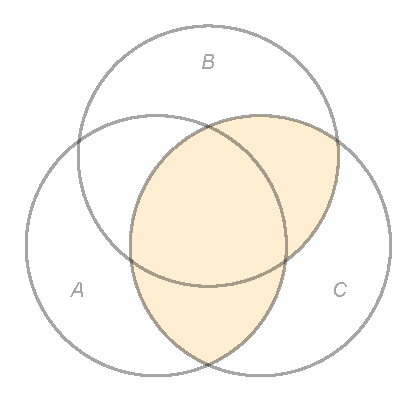
\includegraphics[width=0.2\textwidth]{images/venn1.pdf}}
        =
        \centerimage{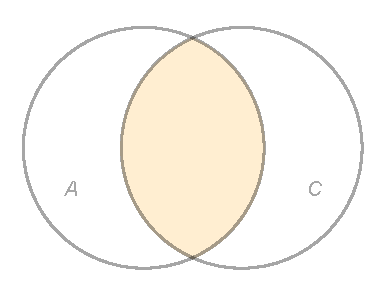
\includegraphics[width=0.2\textwidth]{images/venn2.pdf}}
        \cup
        \centerimage{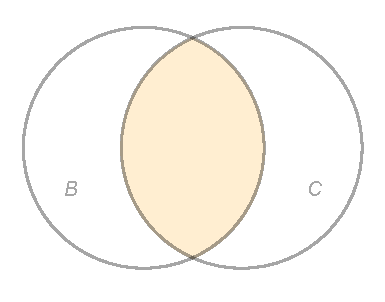
\includegraphics[width=0.2\textwidth]{images/venn3.pdf}}
    \]
    Demonstration of $A \cap \bigcup_{B \in \Gamma} B = \bigcup_{B \in \Gamma}
    (A \cap B)$, with $|\Gamma| = 3$.
    \[
        \centerimage{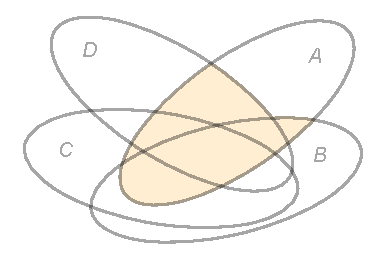
\includegraphics[width=0.2\textwidth]{images/venn4.pdf}} 
        =
        \centerimage{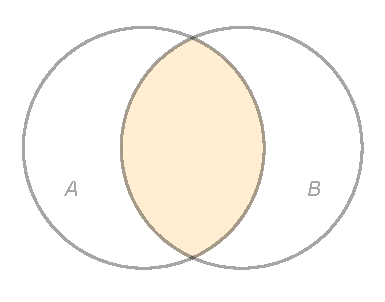
\includegraphics[width=0.2\textwidth]{images/venn5.pdf}} 
        \cup
        \centerimage{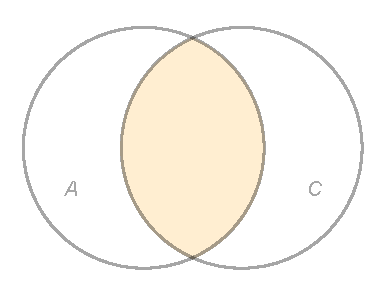
\includegraphics[width=0.2\textwidth]{images/venn6.pdf}} 
        \cup
        \centerimage{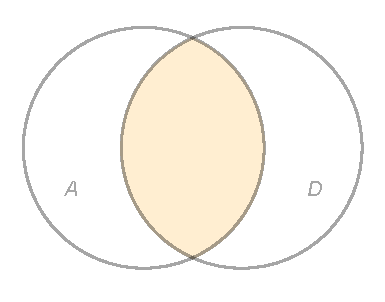
\includegraphics[width=0.2\textwidth]{images/venn7.pdf}} 
    \]
    Demonstration of $A \cup \bigcap_{B \in \Gamma} B = \bigcap_{B \in \Gamma}
    (A \cup B)$, with $|\Gamma| = 3$.
    \[
        \centerimage{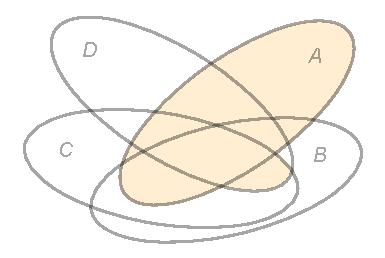
\includegraphics[width=0.2\textwidth]{images/venn11.pdf}} 
        =
        \centerimage{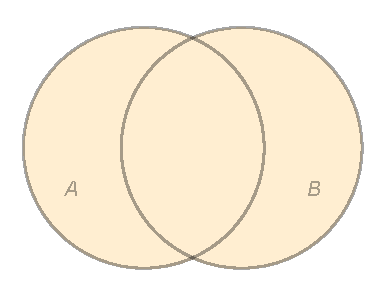
\includegraphics[width=0.2\textwidth]{images/venn8.pdf}} 
        \cap
        \centerimage{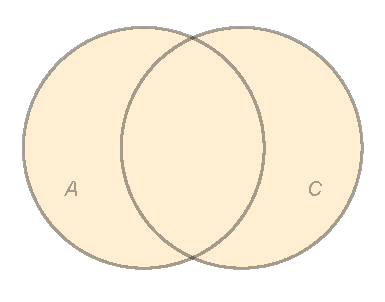
\includegraphics[width=0.2\textwidth]{images/venn9.pdf}} 
        \cap
        \centerimage{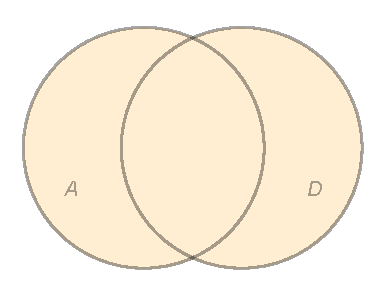
\includegraphics[width=0.2\textwidth]{images/venn10.pdf}} 
    \]
\end{proof}

Primary author: David Kraemer.

\begin{minorEx}[Riddle]%1.9
    Generalize Theorem 1.L to the case of arbitrary collections of sets.
\end{minorEx}

\begin{proof}
    (See 1.N) Let $A$ be a set and let $\Gamma$ be a set consisting of sets,
    then we have 
    $$
    A \cap  \bigcup_{B\in \Gamma} B = \bigcup_{B\in \Gamma} (A \cap B)\text{
    and  } A \cup \bigcap_{B\in \Gamma} B = \bigcap_{B\in \Gamma} (A \cup B)
    $$
\end{proof}
Primary author: Reilly Noonan Grant

\begin{majorEx}[Yet Another Pair of Distributivities]%1.N 
    Let $A$ be a set and let $\Gamma$ be a set consisting of sets, then we have

    $$
    A \cap  \bigcup_{B\in \Gamma} B = \bigcup_{B\in \Gamma} (A \cap B)\text{
    and  } A \cup \bigcap_{B\in \Gamma} B = \bigcap_{B\in \Gamma} (A \cup B)
    $$
\end{majorEx}
\begin{proof}
    We will first show that $A \cap \bigcup_{B\in \Gamma} B = \bigcup_{B\in
    \Gamma} (A \cap B)$ using double containment. 

    First let $x \in A \cap \bigcup_{B\in \Gamma} B$ be arbitrary. We see that
    $$
        x \in A \text{ and } x\in B
    $$ 
    for some $B \in \Gamma$.  We thus know that for some $B$, 
    $$
        x\in (A \cap B)
    $$ 
    We now can see that as 
    $$
        \bigcup_{B\in \Gamma} (A \cap B)
    $$ 
    contains every $(A \cap B)$, we know that 
    $$
        x \in \bigcup_{B\in \Gamma} (A \cap B)
    $$ 
    As $x$ was arbitrary, we know that 
    $$
        A \cap \bigcup_{B\in \Gamma} B \subseteq 
        \bigcup_{B\in \Gamma} (A \cap B).
    $$ 

    We now let $x \in \bigcup (A \cap B)$ be arbitrary.  We see that 
    $$
        x \in A \text{ and } x \in B
    $$ 
    for some $B\in \Gamma$. 
    We also see that as $B\in \Gamma$, that 
    $$
        B \subset \bigcup_{B\in \Gamma} B
    $$ 
    and thus $x \in A \text{ and } x \in \bigcup_{B\in \Gamma}$.  We now can see
    that this only holds if 
    $$
        x \in A \cap \bigcup_{B\in \Gamma}
    $$ 
    and thus as $x$ was arbitrary 
    $$
        A \cap \bigcup_{B\in \Gamma} B \supseteq \bigcup_{B\in \Gamma} (A \cap
        B).
    $$ 
    We now can see by double containment, that $A \cap \bigcup_{B\in \Gamma} B =
    \bigcup_{B\in \Gamma} (A \cap B)$.

    We will now show that 
    $$
        A \cup \bigcap_{B\in \Gamma} B = \bigcap_{B\in \Gamma} (A \cup B)
    $$ 
    by double containment.

    We first let $x \in A \cup \bigcap_{B\in \Gamma} B$ be arbitrary.  We see that 
    $$
        x \in A \text{ or } x \in \bigcap_{B\in \Gamma} B
    $$ 
    We now suppose that $x \in A$. We would then see that $x \in A \cup B$ for
    any $B$, and thus 
    $$
        x \in \bigcap_{B\in \Gamma} (A \cap B)
    $$

    Now suppose that $x \notin A$. We would then see that 
    $$
        x \in \bigcap_{B\in \Gamma} B
    $$ 
    and if $x$ is in some $B$, we know that it would also be in $A
    \cup B$, so thus, we would know that 
    $$
        x \in \bigcap_{B\in \Gamma} (A \cup B)
    $$

    As $x$ was arbitrary, we know that 
    $$
        A \cup \bigcap_{B\in \Gamma} B \subseteq \bigcap_{B\in \Gamma} (A \cup B)
    $$

    We now let $x \in \bigcap_{B\in \Gamma} (A \cup B)$ be arbitrary.
    We can see
    that $x \in A$ or $x \in B$ for every $B \in \Gamma$.  Suppose $x
    \in A$. It would then be the case that $x \in A \cup
    \bigcap_{B\in\Gamma} B$ as $x \in A$.
    Now, suppose that $x \notin A$ we would then have that $x \in
    \bigcap_{B\in\Gamma} B$ as $x \in \bigcap_{B\in\Gamma} (A \cap B)$, and $x
    \notin A$. We thus see that as $x$ was arbitrary, that 
    $$
        A \cup \bigcap_{B\in \Gamma} B \supseteq \bigcap_{B\in \Gamma} (A \cup
        B).
    $$
    and thus 
    $$
        A \cup \bigcap_{B\in \Gamma} B = \bigcap_{B\in \Gamma} (A \cup B)
    $$
    We can now see that
    $$
        A \cap  \bigcup_{B\in \Gamma} B = \bigcup_{B\in \Gamma} (A \cap B)\text{
        and  } A \cup \bigcap_{B\in \Gamma} B = \bigcap_{B\in \Gamma} (A \cup B)
    $$

\end{proof}
Primary author: Reilly Noonan Grant